% Chapter 3

\chapter{Description of the Setup} % Chapter title
\label{ch:setup} % For referencing the chapter elsewhere, use \autoref{ch:mathtest}

This chapter details the setup that was used in the design of a Swept Source OCT system developed for this thesis work, describing the optical and electrical components that were employed. 

\noindent Particular care will be given to the characterization of the \ac{DAQ} board and the design of the acquisition software. 

\section{Optical Source}
As already discussed in \autoref{ch:theory}, \ac{SS-OCT} systems employ a narrow-bandwidth tunable laser to enable a simple detection scheme and is one of the most critical components of the entire system. The source that was used in this thesis is a SSOCT-1310 by Axsun Technologies, which is a class 3 laser that uses a \ac{MEMS} tunable filter to sweep wavelengths in the 1300 nm range. 

The two most important features of this laser are the fast sweep rate, which enables high speed imaging, and the presence of the $k$-clock signal used for equalizing the nonlinear frequency sweep. 

\begin{figure}[bth]
	\myfloatalign
	{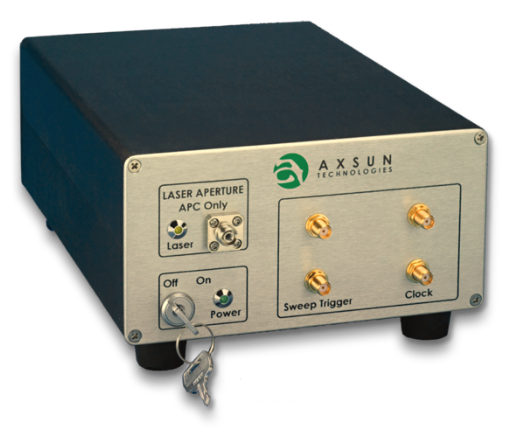
\includegraphics[width=.6\linewidth]{gfx/ch3/axsun}}
	\caption{The acquisition board, AlazarTech ATS9350.}\label{fig:axsun-laser}
\end{figure}

An photo of the laser is available in \autoref{fig:axsun-laser}. The emitted light is collected by connecting a fiber optic patch cord to the FC/APC connector on the front panel, which also includes two SMA connectors for the sweep-start trigger and the $k$-clock signal.


  \begin{table}
	\myfloatalign
	\begin{tabularx}{\textwidth}{Xll} \toprule
		\tableheadline{Parameter} & \tableheadline{Units} & \tableheadline{Value}
		\\ \midrule
		Sweep Rate &  kHz & 100.2 \\
		Center Wavelength & nm & 1305 \\
		Wavelength Tuning Range & nm & 140.38 \\
		Average Power & mW & 25.7 \\
		Duty Cycle & \% & 77.3 \\
		Sampled Duty Cycle & \% & 50.5 \\
		External Clock Min Frequency & MHz & 183.1 \\
		External Clock Average Frequency & MHz & 307.0 \\
		External Clock Max Frequency & MHz & 332.1 \\
		Sampling Clocks & -- & 1536 \\
		\bottomrule
	\end{tabularx}
	\caption{Axsun laser datasheet.}
	\label{tab:axsun-datasheet}
\end{table}

\subsection{Optical Spectrum}
A critical parameter in swept sources for OCT applications is the wavelength interval over which the laser is able to tune. From \autoref{tab:axsun-datasheet}, we can see that the Axsun SSOCT-1310 is centered at $\lambda_0 = 1305$ nm with a bandwidth of $\Delta\lambda = 140.38$ nm. These values were verified by connecting the laser output directly to an \ac{OSA}, measuring its spectrum. 

\begin{figure}[hbt]
	{\myfloatalign
		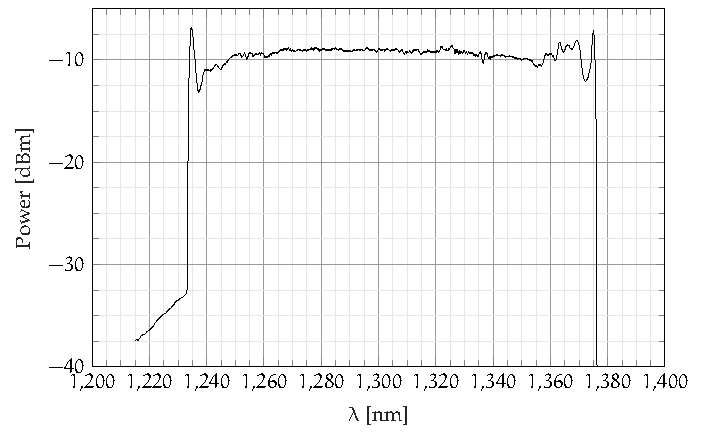
\includegraphics[width=\linewidth]{gfx/tikz/axsun/spectrum}}\\
	\caption{Spectrum of the Axsun SSOCT-1310 laser, obtained with a 1 nm resolution.}\label{fig:axsun-spectrum}
\end{figure}

The measurement was executed with a resolution of 1 nanometer, resulting in the spectrum visible in \autoref{fig:axsun-spectrum}. The edge wavelengths turned out to be $\lambda_1 \approx 1237$ nm and $\lambda_2\approx1376$ nm, which result in a bandwith of $\Delta \lambda \approx 139$ nm and central wavelength of $\lambda_0\approx 1307$ nm. These values slightly differ from those reported in the datasheet, but not enough to compromise the performance of the laser. 

The bandwidth is swept at a frequency $f_a = 100.2$ kHz and with a duty cycle $d_c=0.505$, meaning that the average sweep speed is 
\begin{equation}
\sigma_{\lambda} = \frac{\Delta\lambda f_c}{d_c} \approx 27.8 \,\,\text{nm}/\mu\text{s}.
\end{equation}

Since the goal of SS-OCT sources is to perform a linear frequency sweep, it is more useful to define this parameter in the following manner
\begin{equation}\label{eq:sweep-speed}
\sigma_f = c_0 \left(	\frac{1}{\lambda_0 - \Delta\lambda/2} - \frac{1}{\lambda_0 + \Delta\lambda/2}\right) \frac{f_a}{d_c} \approx 4.9 \,\,\text{THz}/\mu\text{s}
\end{equation}

The istantaneous frequency, after linearization, is thus expressed by 
\begin{equation}
	f(t) = f_0 + \sigma_f t
\end{equation}
where the starting frequency is determined by
\begin{equation}
f_0 = \frac{c_0}{\lambda_0 + \Delta\lambda /2} \approx 218.2 \,\,\text{THz}.
\end{equation}

\subsection{Axial Resolution}
Using \autoref{eq:ss-axial-resolution} and the data provided by \autoref{tab:axsun-datasheet} it is possible to obtain an estimate of the axial resolution provided by the employed optical source. The axial resolution is found to be
\begin{equation}
\delta z \simeq 0.75 \frac{\lambda_0^2}{\Delta \lambda} \approx 9.2 \,\, \mu\text{m.}
\end{equation}

This approximation is valid for sources with a Gaussian spectrum, and can lead to an overestimation of the real axial resolution of the system in case this condition is not met. 

\subsection{Sweep trigger}
The Axsun laser provides a square-wave signal that determines the start of the frequency sweep  and that is used to trigger the acquisition of A-scans. This signal is acquired with a high-speed oscilloscope and illustrated in \autoref{fig:axsun-trigger}. The voltage range was measured as $V_{range} \approx [0 ,1.48] $ V, while the duty cycle is found to be 
\begin{equation}
	d_c = \frac{t_{high}}{t_{high} + t_{low}} \approx 0.97\,.
\end{equation}

For a correct acquisition of A-scans, the datasheet recommends to trigger the acquisition device when the signal level reaches the value of $V_{trig} = 0.71$ V, pictured in \autoref{fig:axsun-trigger} with a red line. 


\begin{figure}[hbt]
	\myfloatalign
	{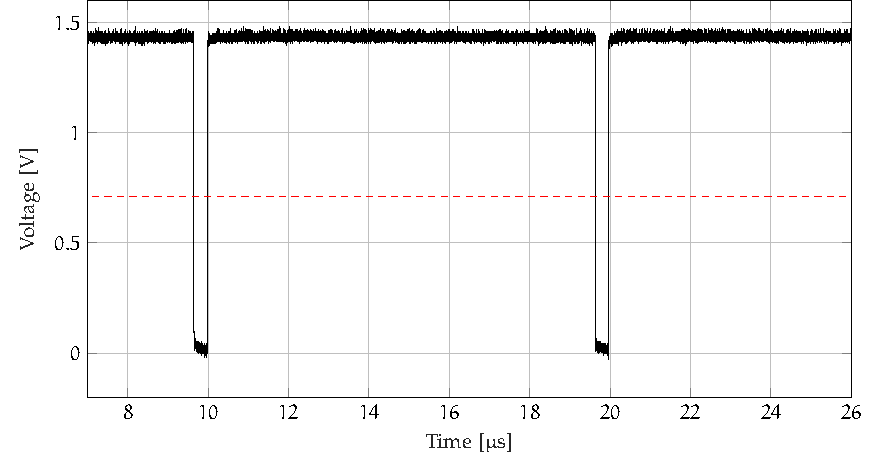
\includegraphics[width=0.8\linewidth]{gfx/ch3/trigger}}\\
	\caption{Sweep trigger of the SSOCT-1310 laser.}\label{fig:axsun-trigger}
\end{figure}

\subsection{Power profile}
Using a photodiode it's possible to measure the istantaneous power profile of the laser emission. The photodiode generates an electrical current which is proportional to the power of the detected electromagnetic field: 
\begin{equation}
	I_{ph} = \mathcal{R} \cdot P 
\end{equation}
The constant $\mathcal{R}$ is called \emph{responsivity} [A/W] and is specific to the detector used. The current can then be measured with an oscilloscope. In order to avoid the saturation of the receiver, a 3 dB coupler was inserted between the source and the photodiode. The obtained power profile is depicted in \autoref{fig:axsun-power} along with the sweep trigger. We can observe that in the first $\sim 5$ $\mu$s after the positive edge of the trigger, the istantaneous power behaves like a typical laser pulse while outside of this interval it assumes an irregular profile. 


\begin{figure}[hbt]
	\myfloatalign
	{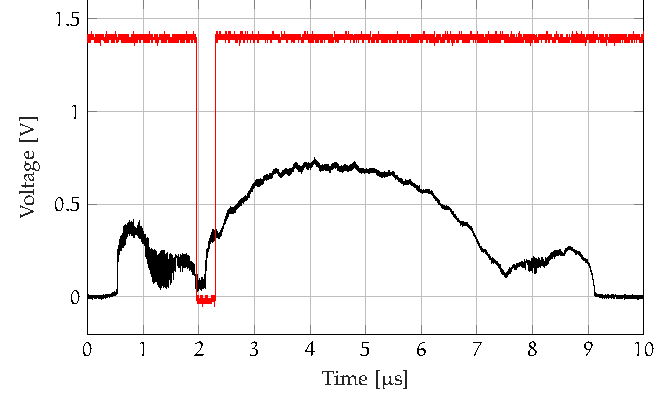
\includegraphics[width=0.8\linewidth]{gfx/ch3/power-profile}}\\
	\caption{Sweep trigger of the SSOCT-1310 laser.}\label{fig:axsun-power}
\end{figure}


\subsection{k-clock}
As already stated, this particular SS-OCT laser is equipped with an internal \ac{MZI} which generates the variable-frequency clock, called $k$-clock, used to sample the A-scan signal at a variable rate and equalize the nonlinear terms in the frequency sweep. As we can see in \autoref{fig:kclock}, this signal assumes values in the $[0, 900]$ mV range with an average value of about 460 mV. This sinusoidal signal will be used to drive the acquisition board for the first $5$ $\mu$seconds of the sweep and from this point forward will be referred to as \emph{useful clock}. As per \autoref{tab:axsun-datasheet}, the total number of samples that cab be acquired using this clock is $N_s = 1536$. In the last 5 $\mu$seconds the clock is called "dummy" because of its undefined behaviour that could lead to issues in the clocking of the DAQ devices.

\begin{figure}[hbt]
	\myfloatalign
	{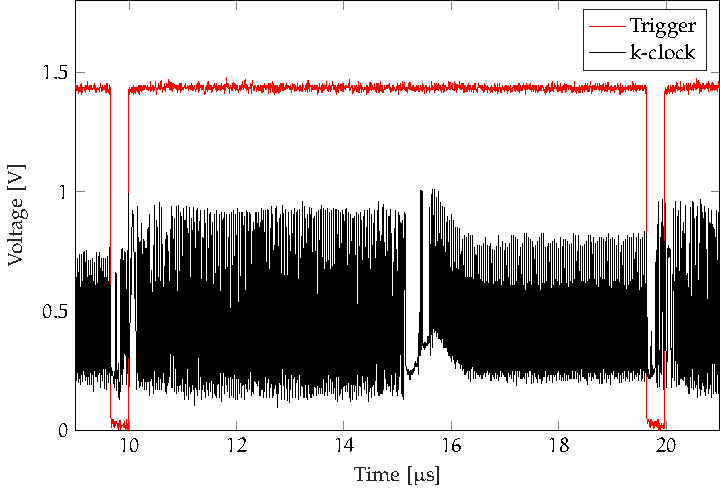
\includegraphics[width=0.8\linewidth]{gfx/ch3/clock}}\\
	\caption{Estimate of the istantaneous frequency of the k-clock.}\label{fig:kclock}
\end{figure}

In \autoref{fig:clock-zoom} are depicted two 50 nanoseconds windows at the start (left) and in the middle (right) of the useful clock, where the variable frequency of signal is clearly visible. Also worth noting is that at the start of the sweep the signal appears much more distorted than in the middle of the sweep. Fortunately, this behaviour did not compromise the performance of the system. 

\begin{figure}[bth]
	\myfloatalign
	{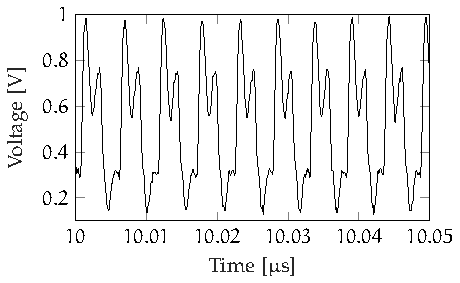
\includegraphics[width=.45\linewidth]{gfx/ch3/clock1}} \quad
	{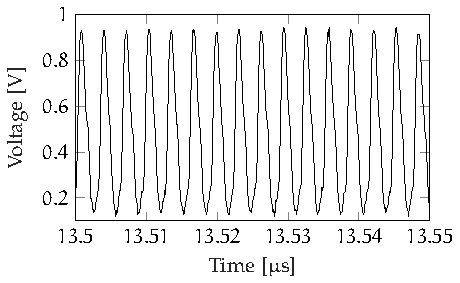
\includegraphics[width=.45\linewidth]{gfx/ch3/clock2}} \\
	\caption{Behaviour of the useful k-clock at different time instants.}\label{fig:clock-zoom}
\end{figure}

To gain further insights on the nature of the frequency sweep, it is interesting to estimate the istantaneous frequency of the k-clock. A method to perform this estimate is the following
\begin{enumerate}
	\item Subtract the average value from the signal
	\item Interpolate the signal $(t, y)$ to obtain $(\hat{t}, \hat{y})$
	\item Determine the time instants $\hat{t}_i$ at which the signal $\hat{y}$ crosses 0, from which a vector $\mathcal{I} = \left[\hat{t}_{i_1}, \hat{t}_{i_2}, \dots,  \hat{t}_{i_N}\right]$ is built.
	\item Compute the difference between the adjacent elements of $\mathcal{I}$ and obtain $\mathcal{T} = \left[\hat{\tau}_{i_1}, \hat{\tau}_{i_2}, \dots,  \hat{\tau}_{i_{N-1}}\right]$,
	\item The istantaneous frequency of the signal is then estimated as $\hat{f}_i = 1/2 \hat{\tau}_i$.
\end{enumerate} 

The result of this method is illustrated in \autoref{fig:kclock-frequency}. Since the estimate is rather noisy, a low pass filter was applied to the $\hat{f}_i$ signal, resulting in a much cleaner estimation (depicted in red). As we can observe, the istantaneous frequency rapidly changes at the start and at the end of the sweep, while in the middle it stabilizes at about 320 MHz. Since a constant k-clock frequency implies a linear frequency sweep, we can infer that the sweep nonlinearities are much more prevalent at the edge of the sampling interval. 

The maximum estimated frequency is $\hat{f}_{clk}^{max} = 339$ MHz, as opposed to the value that was reported in \autoref{tab:axsun-datasheet} of $f_{clk}^{max} = 332.2$ MHz. This slight overestimation is also visible in \autoref{fig:kclock-frequency}, where we can see that the low-pass filtered signal is slightly higher than the average value of the non filtered one.

\begin{figure}[hbt]
	\myfloatalign
	{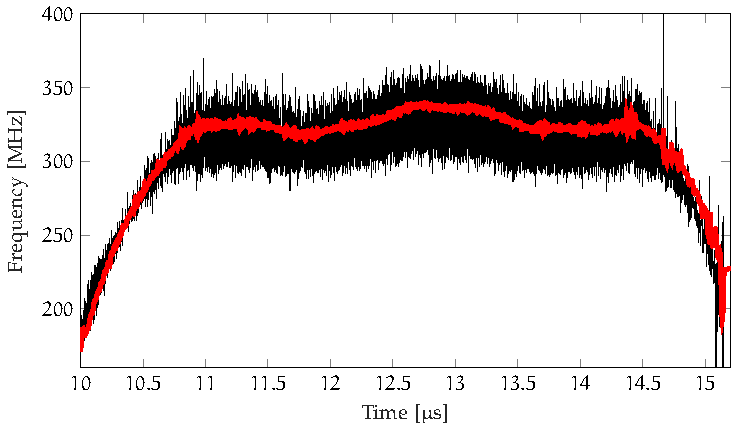
\includegraphics[width=0.8\linewidth]{gfx/ch3/lowpass}}\\
	\caption{Estimate of the istantaneous frequency of the k-clock.}\label{fig:kclock-frequency}
\end{figure}

From the maximum frequency of the k-clock signal we can measure the maximum imaging depth obtainable by the system. 

Two replicas of the pulse overlapping with a relative time delay $\tau$ will generate a beat frequency $f_b$ given by

	\begin{equation}
		f_b = \sigma_f \tau
	\end{equation}
	
where $\sigma_f$, the sweep speed, was determined in \autoref{eq:sweep-speed}. In a OCT setup, the time delay $\tau$ is related to the path mismatch of reference and sample arm, which in turn depends on the depth of the layer of the sample that generates the reflection. In this way	
	\begin{equation}
		\tau = \frac{2dn}{c_0},
	\end{equation}
where $c_0$ is the speed of light in vacuum, $n$ is the refractive index of the sample and $d$ is the depth. By the Nyquist theorem, the maximum beat frequency that can be digitized using the $k$-clock is
	
	\begin{equation}
		f_b^{max} = \frac{f_{clk}^{max}}{2},
	\end{equation}
which results in a maximum depth in air ($n=1$) of  
	\begin{equation}
		d_{max} = \frac{c_0 f_{b}^{max}}{2\sigma_f}  =  \frac{c_0 f_{clk}^{max}}{4\sigma_f} \simeq 5.1 \text{ mm}.
	\end{equation}

\subsection{Coherence length}
In \autoref{ch:theory} we have seen that the coherence length of a source is one of the most important parameters of optical sources, independently of the type of OCT system. In \ac{TD-OCT}, this parameter determines the axial resolution of the system, while \ac{FD-OCT} schemes it also affects the imaging range, as the reference arm is fixed. In particular, complex conjugate artifacts arising from the Fourier trasform of the detected signals halve the maximum imaging range. For this reason, the coherence length of a swept source satisfies the following inequality
\begin{equation}
	l_c \geq 2 \cdot d_{max},
\end{equation}
which implies that the coherence length of the SSOCT-1310 source is at least
\begin{equation}
	l_c \geq 2\cdot d_{max} \approx 10.2 \text{ mm.}
\end{equation}

The exact value was experimentally determined in \cite{Calabrese2017}, measuring the normalized coherence function $|\gamma(\Delta z)|$ by placing a mirror in the sample arm and acquiring the interference signal for different values of \ac{OPD}. The path length difference was changed by translating the reference mirror. The intensity of the interference signal, normalized by its maximum value, is plotted in  \autoref{fig:axsun-coherence-length} as a function of the \ac{OPD}. When the \ac{OPD} increases above a certain value, the coherence function decays exponentially as
\begin{equation}
|\gamma(\Delta z)| \propto e^{-\alpha |\Delta z|},
\end{equation}
which corresponds to a linear decay in the logarithmic domain. The parameter $\alpha$ was estimated by fitting the data points to a line using a Least-Squares fit. The coherence length is finally determined as the $\Delta z$ value such that $|\gamma(\Delta z)| = 1/2$, resulting in
\begin{equation}
	l_c = 2 \cdot \frac{\ln 2}{\alpha} \approx 12.3 \text{ mm.}
\end{equation}


\begin{figure}[hbt]
	\myfloatalign
	{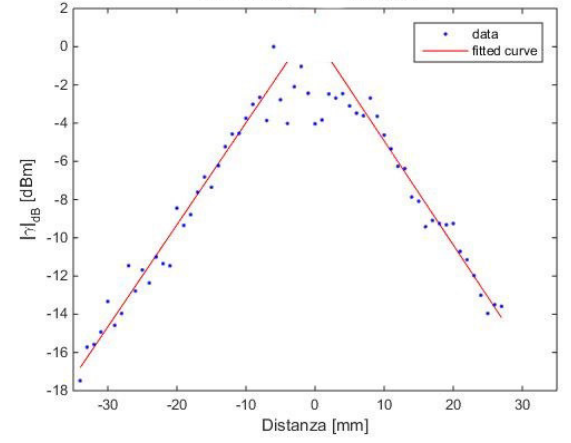
\includegraphics[width=0.8\linewidth]{gfx/ch3/axsun-coherence-length}}\\
	\caption{Experimental estimation of the normalized coherence function.}\label{fig:axsun-coherence-length}
\end{figure}

\section{Scanning System}
One of the most critical components of an OCT is the scanning system. Its role is to receive the light emitted by the source, focus it on the sample under test, and collect the backreflections. A scanning system usually comprises of three different devices

\begin{enumerate}
	\item Fiber collimator
	\item Galvanometric Mirrors
	\item Focusing lens
\end{enumerate}

\begin{figure}[bth]
	\myfloatalign
	{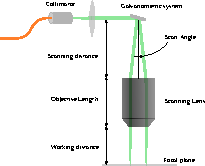
\includegraphics[width=0.8\linewidth]{gfx/setup-diagrams/scanning-diagram.pdf}}
	\caption{Diagram of a OCT scanning system.}\label{fig:scanning-diagram}
\end{figure}

A schematic of this system is depicted in \autoref{fig:scanning-diagram}. Light coming from a single mode optical fiber is deflected by a system of galvanometric mirrors towards a lens which in turns focuses the radiation on the sample. By rotating the mirrors the light beam is focused on a different position on the sample. The reflected beam travels the same path in the opposite direction and is collected by the optical fiber. The correct design of these components is paramount in order to guarantee small transversal and axial resolutions of the OCT system. 



\subsection{Collimator}
The role of the fiber collimator is to collect light coming from a single mode fiber and collimate the beam on the galvanometric mirrors. The divergence angle at the output of the collimator is approximated with the following equation when the beams have a Gaussian intensity profile:
\begin{equation}
	\theta \approx \frac{D}{f} \frac{180}{\pi},
\end{equation}
where $D$ is the mode diameter and $f$ is the focal length of the collimator. This approximation works well for sigle mode fibers, but will underestimate the real divergence angle in the case of multimode fibers, as the intensity profile has a non-Gaussian shape. 

The collimator used in this setup is the Thorlabs F280APC-C\footnote{\url{https://www.thorlabs.com/thorproduct.cfm?partnumber=F280APC-C}}, which is designed to work in the 1310 nm range. Its main specifications are summarized in \autoref{tab:collimator-datasheet}. 

\begin{table}[h]
	\myfloatalign
	\begin{tabularx}{\textwidth}{Xll} \toprule
		\tableheadline{Parameter} & \tableheadline{Units} & \tableheadline{Value}
		\\ \midrule
		Central wavelength & nm & 1310 \\
		Beam diameter & mm & 3.4 \\
		Divergence angle & degrees & 0.028 \\
		Lens numerical aperture (NA) & -- & 0.15 \\
		Focal length & mm & 18.67 \\
		\bottomrule
	\end{tabularx}
	\caption{Thorlabs F280APC-C datasheet.}
	\label{tab:collimator-datasheet}
\end{table}

\subsection{Scanning lens}
The light beam deviated by the galvanometric mirrors has to be focused on the sample under test in order to guarantee high resolution images. This is accomplished by a telecentric focusing lens. This type of lenses is characterized by flat image planes which are ideal for OCT applications. 

The main parameters that characterize this device are the following:
\begin{itemize}
	\item Entrance Pupil Size (EP): it specifies the diameter of the collimated laser beam that will maximize the resolution of the imaging system. When using a single galvanometric mirror, the EP is located at the pivot point of the mirror. When two mirrors are used, the EP is located between the two mirrors. 

	\item Scanning Distance (SD): the distance between the EP and the base of the lens. 
	
	\item Scan Angle (SA): the angle between the incoming light beam and the optical axis of the lens. 
	
	\item Working Distance (WD): the distance between the tip of the lens and the focal plane.
	
	\item Parfocal Distance (PD): the distance between the base of the lens and the focal plane. It is equal to the WD plus the objective length.
	
	\item Field of View (FOV): the area on the focal plane that can be imaged with a resolution equal or better than the one guaranteed by the lens. 
	
	\item Depth of View (DOV): it corresponds to the distance between parallel planes on either side of the focal plane, where the beam spot diameter is $\sqrt{2}$ greater than it is at the focal plane. Using lenses with a high DOV value yields images with high lateral resolution in a larger interval of depths. 
	
	\item Spot size: the diameter of the beam on the focal plane. 
\end{itemize}


 The lens used for the SS-OCT system developed in this thesis is the Thorlabs LSM04\footnote{\url{https://www.thorlabs.com/thorproduct.cfm?partnumber=LSM04}}. Its main specifications are listed in \autoref{tab:lens-datasheet}. A simulation of the beam spot size on the focal plane is available in \autoref{fig:spotsize}, where we can see that it increases for bigger scan angles. This behaviour has the effect of reducing the lateral resolution at the edge of the FOV. 
 
\begin{figure}[bth]
 	\myfloatalign
 	{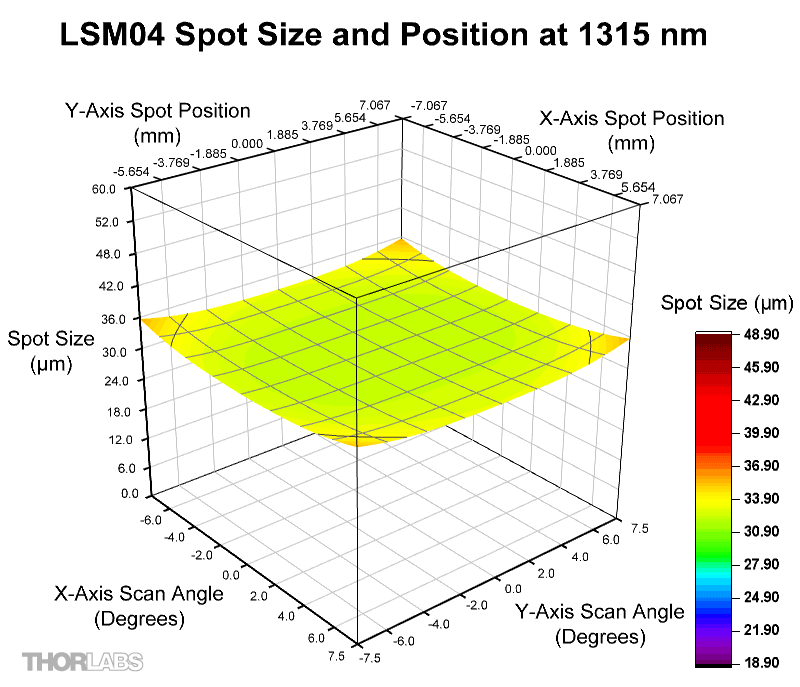
\includegraphics[width=0.6\linewidth]{gfx/ch3/spotsize}}
 	\caption{The Thorlabs GVS002 galvo system.}\label{fig:spotsize}
 \end{figure}
 
 
 
 \begin{table}[h]
 	\myfloatalign
 	\begin{tabularx}{\textwidth}{Xll} \toprule
 		\tableheadline{Parameter} & \tableheadline{Units} & \tableheadline{Value}
 		\\ \midrule
 		Wavelength range & nm & 1250-1380\\
 		Effective Focal Length (EFL) & mm & 54 \\
 		Entrance Pupil size & mm & 4 \\
 		Working Distance & mm & 42.3 \\		
 		Parfocal Distance & mm & 80.8 \\
 		Scan Distance & mm & 18.9 \\
 		Maximum Scan Angle & degrees & $\pm 7.5 \times \pm 7.5$ \\
 		Field of View & mm$^2$ & $14.1 \times 14.1$ \\
 		Depth of View & mm & 0.61\\
 		\bottomrule
 	\end{tabularx}
 	\caption{Thorlabs LSM04 datasheet.}
 	\label{tab:lens-datasheet}
 \end{table}
 
 
 
 \subsubsection{Lateral resolution}
 
 Using the parameters listed in \autoref{tab:lens-datasheet} it is also possible to obtain an estimate of the lateral resolution of the system, which is dictated by the diffraction limited spot size of the focused optical beam. For Gaussian-shaped beams, it is approximated as \cite{Drexler2015}
 \begin{equation}
 	\delta x \simeq \frac{4\lambda_0}{\pi} \frac{f}{d}
 \end{equation}
 where $\lambda_0$ is the central wavelength of operation, $f$ is the focal length of the lens and $d$ is the diameter of the beam at the entrance of the lens. The lateral resolution guaranteed by the LSM04 is thus
 \begin{equation}
 	\delta x \simeq \frac{4\lambda_0}{\pi} \frac{EFL}{EP} \approx 22.5 \,\,\mu\text{m.}
 \end{equation}
 
 Since the diameter of the beam exiting the fiber collimator is slightly smaller ($d=3.4$ mm) than the EP size, the resulting lateral resolution becomes
 \begin{equation}
	\delta x \approx 26.5 \,\,\mu\text{m}.
 \end{equation}
 
 The depth of view, also called confocal parameter, limits the imaging depth of the system. Due to diffraction, this paramer is also governed by the lateral resolution of the system through the following equation
 \begin{equation}
	 b = \frac{2 \delta x^2}{\lambda_0}.
 \end{equation}
 
 This effect is illustrated in \autoref{fig:na}, where we can observe that using lenses with a high numerical aperture (NA), or small spot size, the depth of view is limited. In OCT systems it is preferred to use low NA lenses to sacrifice lateral resolution in favor of a depth of view comparable to the coherence length of the source. Following this criterion the coherence length is fully exploited. 
 
  \begin{figure}[bth]
 	\myfloatalign
 	{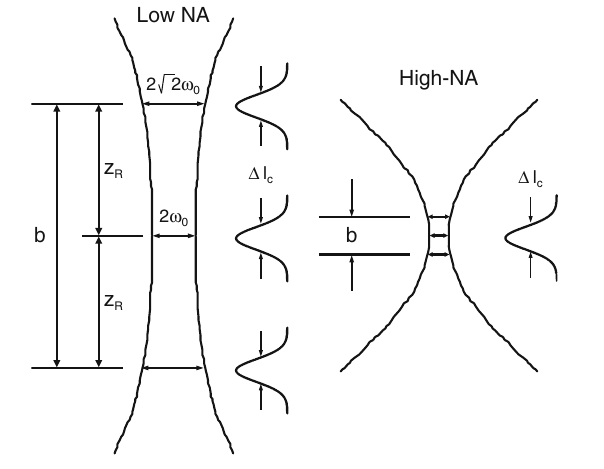
\includegraphics[width=0.6\linewidth]{gfx/ch3/na}}
 	\caption{Basic diagram of a  SS-OCT setup}\label{fig:na}
 \end{figure}
 
 
 Using the EP size the confocal parameter is $b \approx 0.61$ mm, equal to the value reported in \autoref{tab:lens-datasheet}, while using the beam size diameter $d = 3.4$ mm it becomes $b \approx 0.84$ mm. 
 
 

\subsection{Galvanometric Mirrors}

In order to acquire B-scans and C-scans it is necessary to direct the laser beam emitted from the swept laser over a speficied area of the sample. This is accomplished by using a system of \emph{galvanometric mirrors}, also called \emph{galvo mirrors}. A cross-sectional image can be generated with a single 1D mirror, that is, a mirror which can rotate on a single axis, while volumetric data require the use of either a 2D mirror or a couple of 1D mirrors. In the second case, each mirror is responsible for the movement of the beam over a single direction on the focal plane, typically called X and Y. 

\begin{figure}[bth]
	\myfloatalign
	{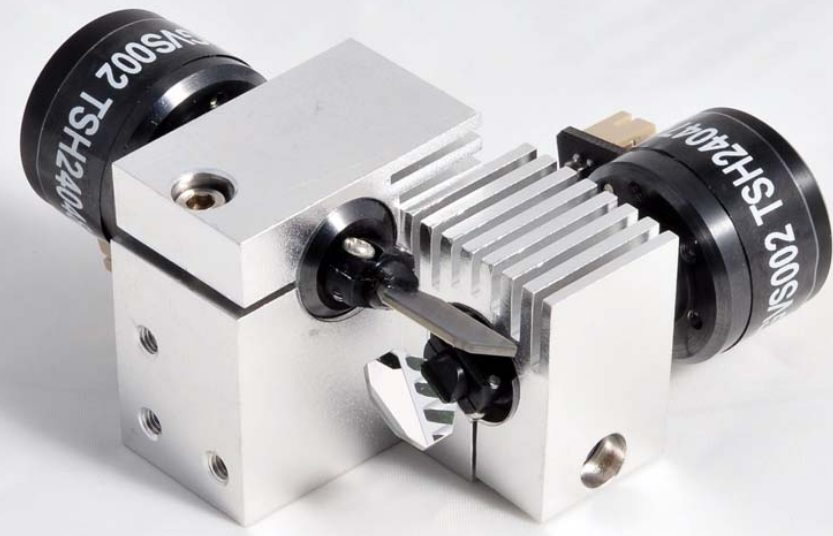
\includegraphics[width=0.6\linewidth]{gfx/ch3/galvo}}
	\caption{The Thorlabs GVS002 galvo system.}\label{fig:galvo}
\end{figure}

The galvo system employed in this thesis work is the Thorlabs GVS002\footnote{\url{https://www.thorlabs.com/thorproduct.cfm?partnumber=GVS002}}, which consists in two 1D silver plated mirrors, the motors that controls them, a detector to measure the mirrors' position  and the servo driver boards that interpret the error signals coming from the detector to correctly drive the motors to the demanded position. A photo of the dual axis motor/mirror assembly is available in \autoref{fig:galvo}. A thorough analysis of the electrical circuitry of the system is found in \cite{Calabrese2017}. 

\subsubsection{Controlling the mirrors}
The position of each mirror is controlled by sending a voltage signal to the respective driver board which is proportional to the mechanical angle of the respective motor. The maximum mechanical scan angle that the GVS002 system can handle is $\pm 12.5^\circ$, but it can vary depending on the laser beam diameter and the voltage scaling factor. This particular galvo system offers three different scaling factors which also govern the maximum input voltage applied to the servo boards:

\begin{center}
\begin{tabularx}{\textwidth}{lll} \toprule
	\tableheadline{Scaling factor} & \tableheadline{Max. voltage} & \tableheadline{Max. scan angle}
	\\ \midrule
	0.5 V/$^\circ$ & $\pm 6.25$ V & $\pm 12.5^\circ$ \\
	0.8 V/$^\circ$ & $\pm 10$ V & $\pm 12.5^\circ$ \\
	1 V/$^\circ$   & $\pm 10$ V & $\pm 10^\circ$ \\
	\bottomrule
\end{tabularx}
\end{center}




The scan angle seen by the focusing lens, called \emph{optical scan angle}, $\theta_o$, is twice the mechanical scan angle applied to the mirror, $\theta_m$. Setting the scaling factor  $\alpha = 1 V/^\circ$, the maximum optical scan angle then becomes $\pm 20^\circ$, which allows us fully exploit the maximum angle supported by the lens. In this case, the full FOV is scanned if the applied voltage is $v_{max} = \pm 7.5^\circ/(2\alpha) = \pm 3.75$ V. 

The beam spot position on the focal plane is related to the mechanical angle applied to the mirrors and the focal length of the lens through the following relation

\begin{align}
	x = EFL \tan(2 \theta_{m,x})\label{eq:focusplane-positionx}\\
	y = EFL \tan(2 \theta_{m,y})\label{eq:focusplane-positiony}
\end{align}

With a scaling factor equal to $\alpha$, the voltage signal $v_{x,y}(t)$ will therefore focus the beam at the following position
\begin{align}
x(t) = EFL \tan\left[2 \alpha_s v_x(t) \frac{\pi}{180}\right]\\
y(t) = EFL \tan\left[2 \alpha_s v_y(t) \frac{\pi}{180}\right]
\end{align}

The two signals $v_x$ and $v_y$ are delivered to the driver boards as two pairs of positive voltage signals, $(v_x^+, v_x^-)$ and $(v_y^+, v_y^-)$. 


\subsubsection{Image distortion}
When using a two-mirror system three different effects can appear
\begin{enumerate}
	\item The arrangement of the mirrors leads to a distortion of the image field, which will be "pillow-shaped" instead of rectangular (fig:galvo-distortion). This is due to the fact that the distance between the two mirrors depends on the mechanical angle applied to the mirrors. 
	
	
	\begin{figure}[bth]
		\myfloatalign
		{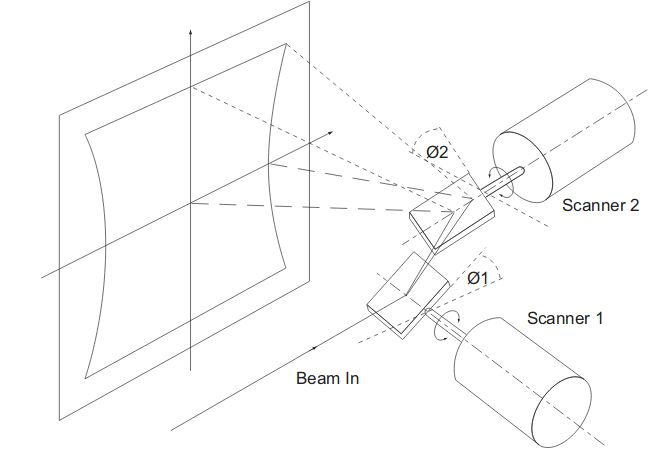
\includegraphics[width=0.75\linewidth]{gfx/ch3/galvo-distortion}}
		\caption{Field distortion using two mirrors.}\label{fig:galvo-distortion}
	\end{figure}
	
	
	\item From \autoref{eq:focusplane-positionx} and \autoref{eq:focusplane-positiony} we can observe that the distance on the image field is not directly proportional to the applied angle but to its tangent. This can result in an additional distortion effect. 
	
	\item If an ordinary lens is used for focusing the laser beam, the focus lies on a sphere.
	In a flat image field, a varying spot size results. 
\end{enumerate}


\begin{figure}[bth]
	\myfloatalign
	{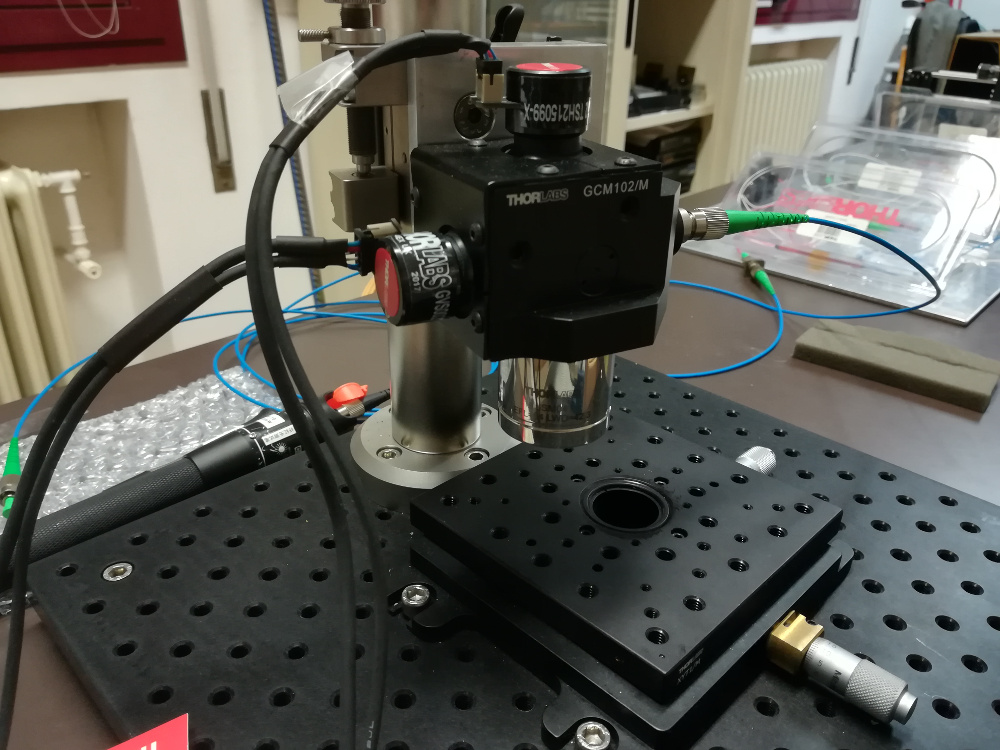
\includegraphics[width=0.75\linewidth]{gfx/ch3/testa}}
	\caption{The final scanning system mounted on a movable vertical support.}\label{fig:testa}
\end{figure}
	
\section{Acquisition Board}

    \begin{figure}[bth]
    \myfloatalign
    {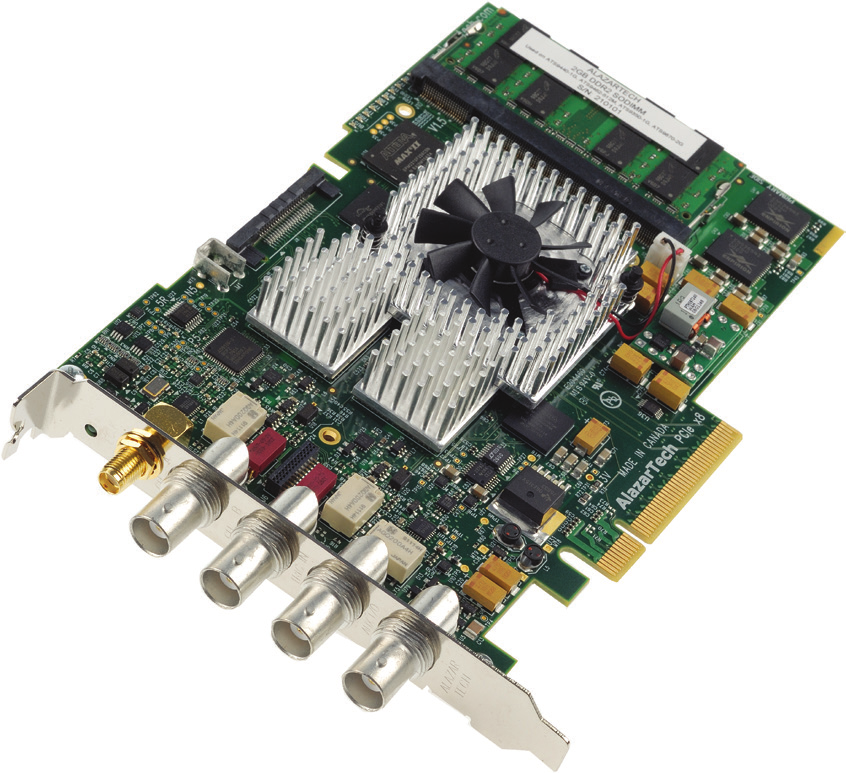
\includegraphics[width=.6\linewidth]{gfx/board}}
    \caption{The acquisition board, AlazarTech ATS9350.}\label{fig:acq-board}
    \end{figure}
	\subsection{}

    \begin{figure}[bth]
    \myfloatalign
    \subfloat[Acquisition using Single-Port Memory.]
    {\label{fig:single-port-acq}
    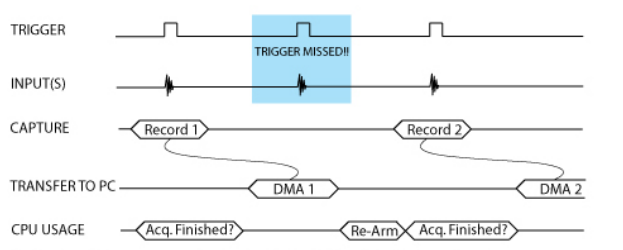
\includegraphics[width=.75\linewidth]{gfx/single-port-acq}} \\
    \subfloat[Acquisition using Dual-Port Memory.]
    {\label{fig:dual-port-acq}
    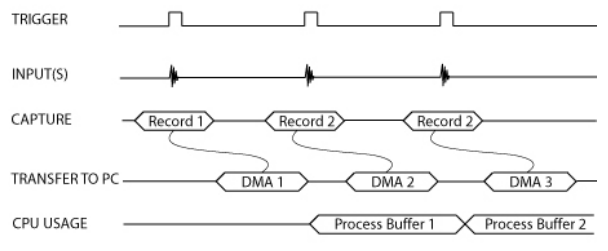
\includegraphics[width=.75\linewidth]{gfx/dual-port-acq}}
    \caption{Diagram highlighting the differences between Sigle-Port acqusitions and Dual-Port acqusitions}\label{fig:single-vs-dual-port}
    \end{figure}

    In \autoref{fig:single-vs-dual-port} a comparison between the two acquisition techniques is available. For Single-port Acquisitions, in \autoref{fig:dual-port-acq} we can see that no trigger events are missed and over 95\% of CPU time is available for data processing, while in \autoref{fig:single-port-acq} trigger events happening while the DMA transfer is ongoing are missed completely, and virtually all CPU cycles are used in managing the data acquisition. This leaves no room for data processing on the CPU. 
    


\section{Optical Circuit}

\subsection{ Mach-Zender Interferometer }
In order to test the k-clock and the acquisition device blah blah blah used AlazarDSO softeare to obtani the beating signal of unbalanced MZI -> show difference also on images
\begin{figure}[bth]
	\myfloatalign
	{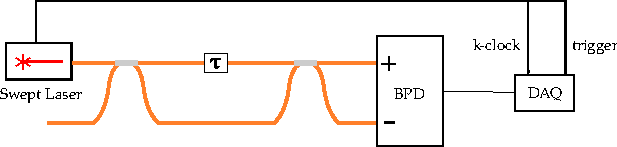
\includegraphics[width=\linewidth]{gfx/setup-diagrams/interferometer.pdf}}
	\caption{Diagram of an unbalanced Mach-Zender Interferometer.}\label{fig:unbalanced-mzi}
\end{figure}

\subsection{Basic setup and Stability Analysis}


\subsection{Final Setup with OBR balancing}
Add couplers length measurements;  focus in the middle of the imaging range. 

\subsection{Axial Resolution}
Try with new measurements

\subsection{Thickness measurements}
No scattering detected, only reflections caused by the surface


\begin{figure}[hbt]
\myfloatalign
{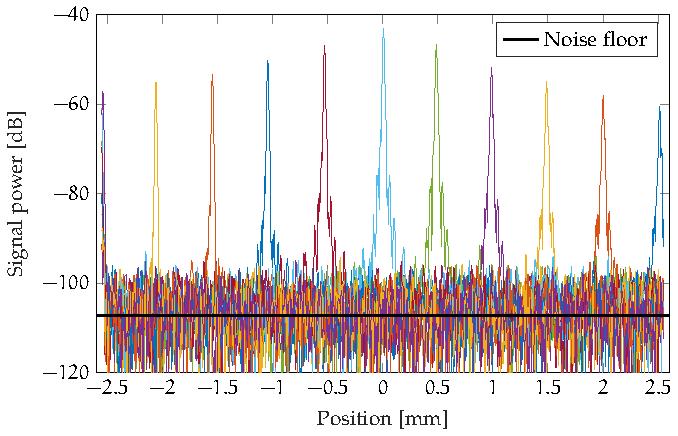
\includegraphics[width=\linewidth]{gfx/falloff}}
\caption{Signal spectrum at various depths.}\label{fig:power-falloff}
\end{figure}


\begin{figure}[hbt]
\myfloatalign
{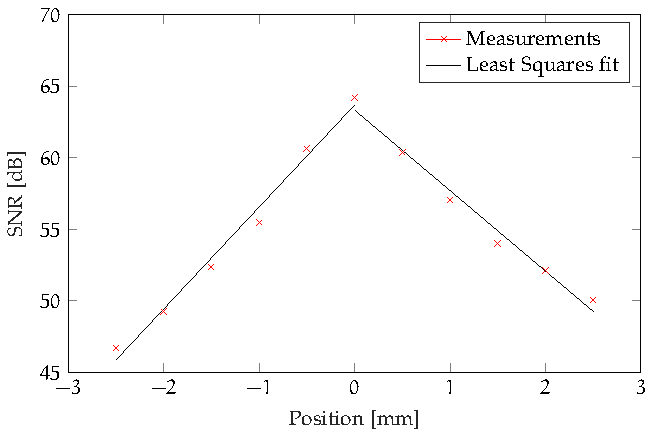
\includegraphics[width=0.9\linewidth]{gfx/falloff-fit}}
\caption{Signal-to-noise ratio falloff.}\label{fig:falloff-fit}
\end{figure}



\begin{figure}[hbt]
\centering
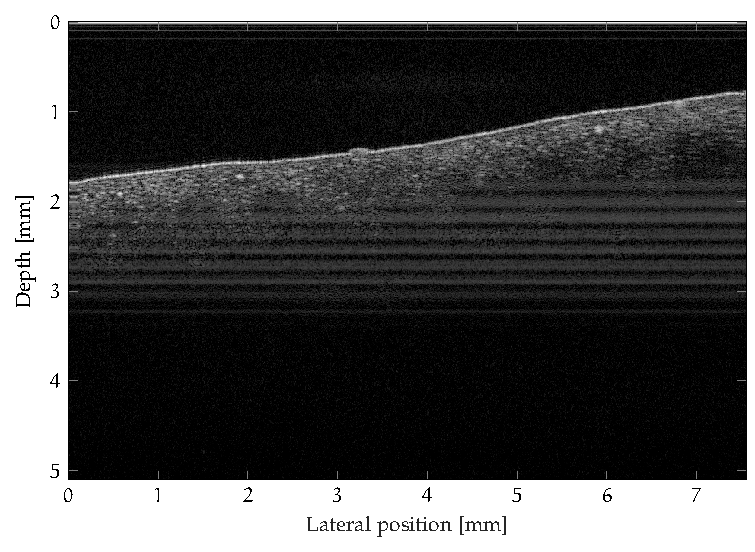
\includegraphics[width=\linewidth]{gfx/tikz/axsun/banana-peel}
\caption{B-scan of banana peel.}\label{fig:banana-peel}
\end{figure}%----------------------------------------------------------------------------------------
\begin{figure}[hbt]
\myfloatalign
{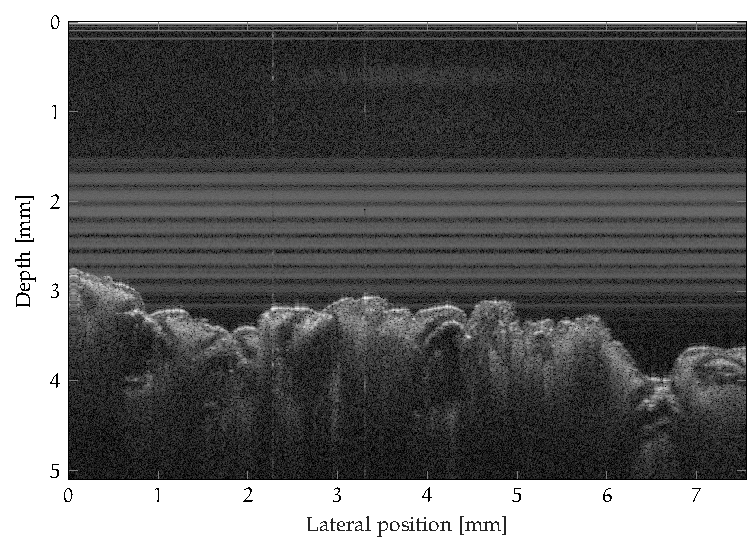
\includegraphics[width=\linewidth]{gfx/tikz/axsun/dry-orange-peel}}
\caption{B-scan of dry orange peel.}\label{fig:dry-orange-peel}
\end{figure}%----------------------------------------------------------------------------------------

\begin{figure}[hbt]
\myfloatalign
{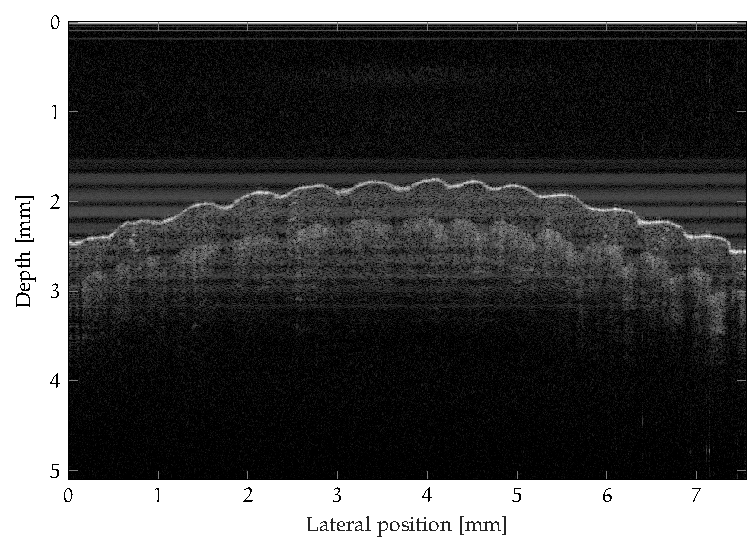
\includegraphics[width=\linewidth]{gfx/tikz/axsun/finger}}
\caption{B-scan of a human finger.}\label{fig:finger}
\end{figure}%----------------------------------------------------------------------------------------
%----------------------------------------------------------------------------------------
